\section{Experiments}
\label{appendix:experiments}
In this section, we empirically validate our theoretical framework. A key challenge in evaluating reject-option strategies based on regret is that the calculation of \textit{True Regret} requires access to the true data-generating process $p(y|x, \theta_*)$, which is unknown for real-world datasets.

To address this, we construct a controlled high-dimensional setup that allows us to generate realistic image data while maintaining full access to the ground-truth data-generating process. This enables the exact computation of the Bayes-optimal prediction, the true regret and the true aleatoric uncertainty for every sample, allowing us to benchmark the proposed epistemic reject-option against standard baselines.

\paragraph{Important Note:} This synthetic generation is strictly for validation purposes to verify \Cref{thm:EpistemicRejOpt}. In practice, the proposed Epistemic Reject-Option predictor ($Q_E$) relies only on the learned posterior and does \textbf{not} require knowledge of the ground truth for inference. Only the evaluation of the regret requires access to the data-generating process $p(y|x, \theta_*)$.

\subsection{Experimental Setup}
\paragraph{Data Generation} We define the input distribution $p(x)$ using StyleGAN3 \cite{Karras2021} trained on the Flickr-Faces-HQ Dataset (FFHQ) dataset, which generates high-quality synthetic face images. To define the conditional distribution $p(y|x)$, we create a \textit{Ground-Truth Generator} as follows:
\begin{enumerate}
    \item We train a ViT-B-16 age estimation model on all publicly available age estimation datasets using cross-entropy loss.
    \item We distill the model into a ResNet-50 regression network. This network acts as the oracle: for any input $x$, it outputs a ground-truth mean $\mu_*(x)$ and variance $\sigma^{2}_*(x)$.
    \item Our data generation process is thus defined as $y \mid x \sim \mathcal{N}(\mu_*(x), \sigma_*^{2}(x))$.
\end{enumerate}

For our experiments, we sample a test set of $100,000$ images from $p(x)$. Training sets of varying sizes $m$ are generated by sampling $x \sim p(x)$ and labeling them by sampling a single target $y$ from the $p(y|x)=\mathcal{N}(\mu_*(x), \sigma^{2}_*(x))$.

\paragraph{Models and Training} We employ Bayesian Linear Regression (BLR) as the learning algorithm, implemented as a Gaussian Process with a linear kernel. The learner operates on a fixed feature representation $\phi(x)$ of the input image. We compare three reject-option strategies:
\begin{enumerate}
    \item \textbf{Aleatoric:} Rejects inputs with high irreducible noise using either the true $A_*(x, D)=\sigma_*^2(x)$ or its estimate.
    \item \textbf{Total:} Rejects based on $T_*(x, D)$, the variance of the predictive distribution.
    \item \textbf{Epistemic:} Rejects based on the expected conditional regret $E_*(x, D)$.
\end{enumerate}
    
We employ the Area under the Regret-Coverage Curve and the Area under the Risk-Coverage Curve as our metrics. Risk and regret are calculated using the squared loss.

\subsection{Validation on Well-Specified Models}
We first investigate the setting where the learner is well-specified, meaning the ground-truth function lies within the hypothesis class of the learner. To achieve this, we use the penultimate layer features of the Ground-Truth Generator, the ResNet-50 used to define $p(y|x)$, as the input features $\#\phi(x)\in\mathbb{R}^d$, $d=2048$, for the Bayesian Linear Regressor.

\paragraph{Oracle Aleatoric Variance} Initially, we provide the learner with the true aleatoric variance $\sigma^{2}_*(x)$ to isolate the behavior of the uncertainty estimates. \Cref{fig:oracle_resnet_gp_linear} displays the performance. The proposed Epistemic strategy (red) consistently achieves the lowest Area under Regret Coverage across all sample sizes, empirically confirming that $E_*(x, D)$ is the optimal ranking function for minimizing regret. Conversely the Aleatoric strategy (blue) minimizes Risk. This confirms the theoretical distinction: the Epistemic predictor accepts noisy samples if the model has learned the mean accurately (low regret, high risk), whereas the Aleatoric predictor rejects them.

\begin{figure}[htb]
    \centering
    \begin{minipage}[t]{0.48\linewidth}
        \centering
        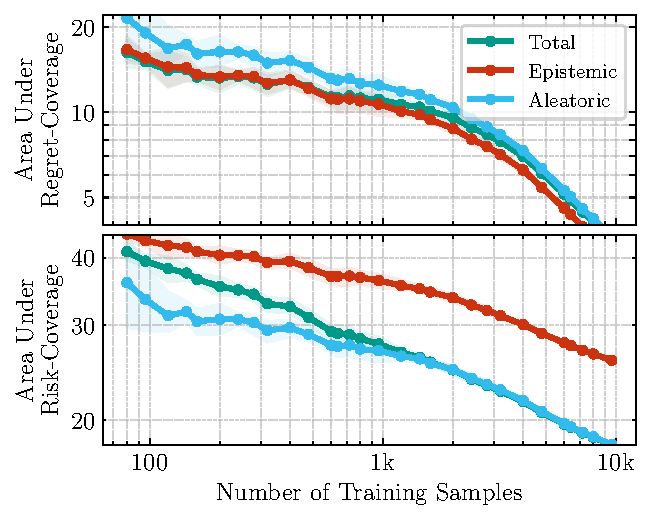
\includegraphics[width=\linewidth]{figures/oracle_resnet_gp_linear.pdf}
        \caption{Performance comparison in the well-specified setting using oracle aleatoric variance. The top row shows the Area Under Regret-Coverage, and the bottom row shows the Area Under Risk-Coverage. As predicted by the theory, the Epistemic reject-option (red) consistently minimizes regret, while the Aleatoric reject-option (blue) minimizes risk. The Total uncertainty (green) acts as an interpolation: in the low-data regime, it is dominated by epistemic uncertainty and follows the red curve; as sample size increases, epistemic uncertainty vanishes, and it converges to the aleatoric behavior (blue curve).}
        \label{fig:oracle_resnet_gp_linear}
    \end{minipage}
    \hfill
    \begin{minipage}[t]{0.48\linewidth}
        \centering
        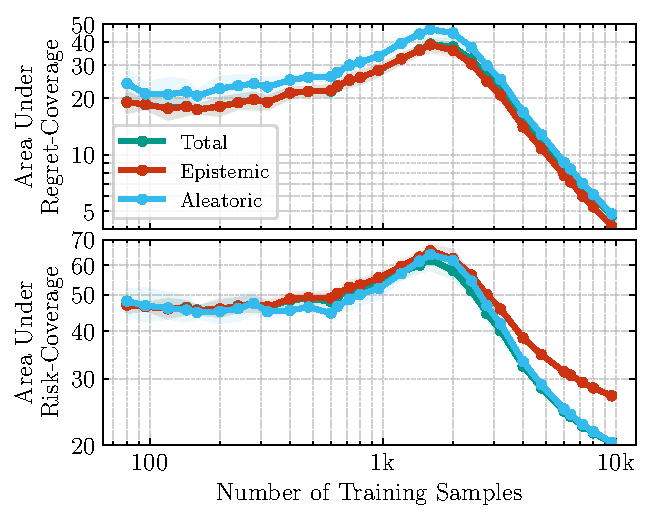
\includegraphics[width=\linewidth]{figures/standard_resnet_gp_linear.pdf}
        \caption{Performance comparison in the well-specified setting using learned aleatoric variance. Here, the noise parameter $\sigma^2$ is estimated via MLE. A characteristic peak in error appears around the interpolation threshold ($|D| \approx d = 2048$). In the under-determined regime ($|D| < 2048$), where the noise estimate often collapses to zero, the Epistemic reject-option (red) remains robust, consistently achieving the lowest regret. This confirms that the posterior variance $E_*(x, D)$ can serve as a proxy for model error even when noise estimation is unstable.}
        \label{fig:resnet_gp_linear}
    \end{minipage}
\end{figure}

\paragraph{Learned Aleatoric Variance} In a realistic setting, $\sigma^{2}_*(x)$ is unknown. We train separate linear layers to estimate the mean $\hat{\mu}(x)$ and noise variance $\hat{\sigma}^2(x)$ via Maximum Likelihood Estimation and use this variance estimate to calibrate the BLR. \Cref{fig:resnet_gp_linear} presents the results. We observe a distinct behavior around $|D| \approx 2048$ samples ($|D| \approx d$). In the under-determined regime ($|D| < d$), the linear model is capable of perfectly interpolating the training data. Consequently, the MLE estimate for the aleatoric variance $\hat{\sigma}^2$ collapses toward zero, effectively leading the learner to treat the data as noiseless. As $|D|$ approaches $d$, the model transitions from interpolation to regression, resulting in the characteristic \textit{double descent} peak in risk and regret due to the ill-conditioning of the covariance matrix. Notably, despite the variance estimate collapsing in the low-data regime and the spectral instability at the interpolation threshold, the Epistemic reject-option maintains the property of minimizing regret. This demonstrates that the posterior variance of the weights $E_*$(x, D) remains a robust signal for model error, even when the aleatoric noise estimate is unreliable.

\subsection{Limitations under Model Misspecification}
We further investigate a \textit{misspecified} setting where the ground-truth function lies outside the hypothesis class. We replicate the experimental setup using FaRL features \cite{Zheng_2022_CVPR}, rendering the true function $\mu_*(x)$ non-linear with respect to the linear Bayesian predictor. In this regime, as $|D| \to \infty$, the parameter posterior concentrates around a single linear approximation. Consequently, the epistemic uncertainty vanishes, yet the regret converges to a non-zero constant corresponding to the approximation error (bias). This reveals a fundamental property: the proposed epistemic reject-option specifically targets \textit{estimation error} (finite data) rather than \textit{approximation error} (limited capacity). Notably, preliminary investigations suggest this behavior is not unique to the linear setting; we observed similar results with Gaussian Processes with RBF kernel and Deep approximations (MC Dropout, Deep Ensembles), highlighting an open challenge for the field.

%%%%%%%%%%%%%%%%%%%%%%%%%%%%%%%%%%%%%%%%%%%%%%%%%%%%%%%%%%%%%%%%%
\section{Proof of Theorem~\ref{equ:BayesianRejOpt}}
\label{appendix:ProofBayesianRejOpt}
%%%%%%%%%%%%%%%%%%%%%%%%%%%%%%%%%%%%%%%%%%%%%%%%%%%%%%%%%%%%%%%%%


The proof of Theorem~\ref{equ:BayesianRejOpt} is standard; we include it here for completeness and to keep the paper self-contained.

\begin{proof}The goal is to determine a base predictor
\(H \colon \SX \times (\SX \times \SY)^m \rightarrow \SY\)
and a selector \(C \colon \SX \times (\SX \times \SY)^m \rightarrow \{0,1\}\),
which together define a reject-option predictor
\(Q = (H,C)\) (cf.~\eqref{equ:BLRejectOptionPred}),
that minimizes the objective
\[
R_{\varepsilon}(H,C)
=
\EE_{(x,D)\sim p(x,D)}
\Big[
C(x,D)\,T(x,D)
+
\bigl(1 - C(x,D)\bigr)\,\varepsilon
\Big],
\]
where
\[
T(x,D)
=
\EE_{y\sim p(y \mid x,D)}
\bigl[
\ell\bigl(y, H(x,D)\bigr)
\bigr].
\]
%
Since the expectation decomposes over pairs \((x,D)\), the optimization can be carried out independently for each \((x,D)\). We therefore fix an arbitrary \((x,D)\) and proceed in two steps.

\medskip
\noindent
\textbf{Step 1: Optimization w.r.t. \(H(x,D)\).}
Assume that \(C(x,D)\) is fixed.
The contribution of \((x,D)\) to \(R_{\varepsilon}(H,C)\) is then
\[
C(x,D)\,
\EE_{y\sim p(y \mid x,D)}
\bigl[
\ell(y,H(x,D))
\bigr]
+
\bigl(1 - C(x,D)\bigr)\,\varepsilon .
\]
Since the second term does not depend on \(H(x,D)\), the optimal predictor is given by
\[
H_*(x,D)
=
\argmin_{\hat y \in \SY}
\EE_{y\sim p(y \mid x,D)}
\bigl[
\ell(y,\hat y)
\bigr],
\]
which coincides with the optimal Bayesian predictor defined in~\eqref{equ:BLOptBayes}.


\medskip
\noindent
\textbf{Step 2: Optimization w.r.t. \(C(x,D)\).}
Now fix \(H(x,D) = H_*(x,D)\).
The remaining optimization problem reduces to
\[
\argmin_{\hat c \in \{0,1\}}
\Big[
\hat c\,T_*(x,D)
+
(1-\hat c)\,\varepsilon
\Big],
\]
where
\(
T_*(x,D)
=
\EE_{y\sim p(y \mid x,D)}
[
\ell(y, H_*(x,D))
]
\).
The optimal selector is therefore
\[
C_T(x,D)
=
\begin{cases}
1, & \text{if } \;\; T_*(x,D) \le \varepsilon, \\
0, & \text{if } \;\;T_*(x,D) > \varepsilon .
\end{cases}
\]
Equivalently,
\(C_T(x,D) = \one{T_*(x,D) \le \varepsilon}\).

Combining the two steps yields the claimed form of the optimal Bayesian reject-option predictor, $Q_B=(H_*,C_T)$.
%
\end{proof}

%%%%%%%%%%%%%%%%%%%%%%%%%%%%%%%%%%%%%%%%%%%%%%%%%%%%%%%%%%%%%%%%%
\section{Proof of Theorem~\ref{thm:EpistemicRejOpt}}
%%%%%%%%%%%%%%%%%%%%%%%%%%%%%%%%%%%%%%%%%%%%%%%%%%%%%%%%%%%%%%%%%
\label{appendix:ProofOfEpistemicTheorem}

The proof of Theorem~\ref{thm:EpistemicRejOpt} follows the same structure as the proof of Theorem~\ref{equ:BayesianRejOpt} given in Appendix~\ref{appendix:ProofBayesianRejOpt}. The key difference lies in the objective, which is based on expected regret rather than expected risk.

\begin{proof}
The goal is to determine a base predictor
\(H \colon \SX \times (\SX \times \SY)^m \rightarrow \SY\)
and a selector
\(C \colon \SX \times (\SX \times \SY)^m \rightarrow \{0,1\}\),
which together define a reject-option predictor
\(Q = (H,C)\) (cf.~\eqref{equ:BLRejectOptionPred}),
that minimizes the objective
\[
R_{\delta}(H,C)
=
\EE_{(x,D)\sim p(x,D)}
\Big[
C(x,D)\,E(x,D)
+
\bigl(1 - C(x,D)\bigr)\,\delta
\Big],
\]
where
\[
E(x,D)
=
\EE_{(\theta,y)\sim p(\theta,y \mid x,D)}
\bigl[
\ell\bigl(y, H(x,D)\bigr)
-
\ell\bigl(y, h(x,\theta)\bigr)
\bigr].
\]

Since the expectation decomposes over pairs \((x,D)\), the optimization can be carried out independently for each \((x,D)\).
We therefore fix an arbitrary \((x,D)\) and proceed in two steps.

\medskip
\noindent
\textbf{Step 1: Optimization w.r.t. \(H(x,D)\).}
Assume that \(C(x,D)\) is fixed.
The contribution of \((x,D)\) to \(R_{\delta}(H,C)\) is then
\[
C(x,D)\,
\EE_{(\theta,y)\sim p(\theta,y \mid x,D)}
\bigl[
\ell(y,H(x,D)) - \ell(y,h(x,\theta))
\bigr]
+
\bigl(1 - C(x,D)\bigr)\,\delta .
\]
Since the second term and the \(\EE_{\theta,y}[\ell(y,h(x,\theta))]\) do not independent of \(H(x,D)\),
the optimal predictor is given by
\[
H_*(x,D)
=
\argmin_{\hat y \in \SY}
\EE_{(\theta,y)\sim p(\theta,y \mid x,D)}
\bigl[
\ell(y,\hat y)
\bigr]
=
\argmin_{\hat y \in \SY}
\EE_{y\sim p(y \mid x,D)}
\bigl[
\ell(y,\hat y)
\bigr].
\]
Thus, \(H_*(x,D)\) coincides with the optimal Bayesian predictor defined in~\eqref{equ:BLOptBayes}.

\medskip
\noindent
\textbf{Step 2: Optimization w.r.t. \(C(x,D)\).}
Now fix \(H(x,D) = H_*(x,D)\).
The remaining optimization problem reduces to
\[
\argmin_{\hat c \in \{0,1\}}
\Big[
\hat c\,E_*(x,D)
+
(1-\hat c)\,\delta
\Big],
\]
where
\(
E_*(x,D)
=
\EE_{(\theta,y)\sim p(\theta,y \mid x,D)}
\bigl[
\ell(y,H_*(x,D)) - \ell(y,h(x,\theta))
\bigr]
\).
The optimal selector is therefore
\[
C_E(x,D)
=
\begin{cases}
1, & \text{if }\;\; E_*(x,D) \le \delta, \\
0, & \text{if }\;\; E_*(x,D) > \delta .
\end{cases}
\]
Equivalently,
\(C_E(x,D) = \one{E_*(x,D) \le \delta}\).

Combining the two steps yields the claimed form of the optimal epistemic reject-option predictor.

\end{proof}


%%%%%%%%%%%%%%%%%%%%%%%%%%%%%%%%%%
\section{Derivation of Epistemic Uncertainty for Specific Loss Functions}
%%%%%%%%%%%%%%%%%%%%%%%%%%%%%%%%%%


Table~\ref{tab:Summary} summarizes special instances of the Bayesian predictor \(H_*(x,D)\), the total uncertainty \(T_*(x,D)\), and the epistemic uncertainty \(E_*(x,D)\) for three commonly used loss functions: squared loss, 0/1 loss, and cross-entropy loss. Throughout the paper, we assume that the parametric model of the data factorizes as
\[
p(x,y \mid \theta) = p(x)\,p(y \mid x,\theta),
\]
so that the predictive distribution takes the form
\[
p(y \mid x,D)
=
\EE_{\theta \sim p(\theta \mid D)}
\bigl[
p(y \mid x,\theta)
\bigr].
\]
This assumption allows several key quantities to be expressed in a simplified and unified manner.


The Bayesian predictor is given by
\[
H_*(x,D)
=
\argmin_{\hat y \in \SY}
\EE_{\theta \sim p(\theta \mid D)}
\Big[
\EE_{y \sim p(y \mid x,\theta)}
\bigl[
\ell(\hat y,y)
\bigr]
\Big].
\]

The total uncertainty associated with this predictor is
\[
T_*(x,D)
=
\EE_{y \sim p(y \mid x,D)}
\bigl[
\ell\bigl(H_*(x,D),y\bigr)
\bigr]
=
\EE_{\theta \sim p(\theta \mid D)}
\Big[
\EE_{y \sim p(y \mid x,\theta)}
\bigl[
\ell\bigl(H_*(x,D),y\bigr)
\bigr]
\Big].
\]

The epistemic uncertainty, measured via the conditional regret, is defined as
\[
E_*(x,D)
=
\EE_{\theta \sim p(\theta \mid D)}
\Big[
\EE_{y \sim p(y \mid x,\theta)}
\bigl[
\ell\bigl(H_*(x,D),y\bigr)
-
\ell\bigl(h(x,\theta),y\bigr)
\bigr]
\Big].
\]

Finally, recall that the Bayes-optimal predictor corresponding to a fixed parameter value \(\theta\) is given by
\[
h(x,\theta)
=
\argmin_{\hat y \in \SY}
\EE_{y \sim p(y \mid x,\theta)}
\bigl[
\ell(\hat y,y)
\bigr].
\]

%%%%%%%%%%%%%%%%%%%%%%%%%%%%%%%%%%
%%%%%%%%%%%%%%%%%%%%%%%%%%%%%%%%%%
\subsection{Squared loss}

Let $\ell(y,\hat{y})=(y-\hat{y})^2$ denote the  squared loss defined over the target space $\SY=\Re$. 

The Bayes-optimal predictor given the true parameter $\theta$ reads:
\[ h_*(x,\theta) = 
  \argmin_{\hat{y}\in\SY}\EE_{y\sim p(y\mid x,\theta)} (y-\hat{y})^2 = \EE_{y\sim p(y|x,\theta)}\big[ y\big ] = \mu_{y|x,\theta}\:.      
\]
The Bayesian predictor:
\begin{eqnarray*}
   H_*(x,D) &= &
\argmin_{\hat{y}\in\SY} \EE_{\theta\sim p(\theta|D)} \Big [\EE_{y\sim p(y|x,\theta)}\big[ (\hat{y}-y)^2 \big ]\Big ]    \\
   &=& \argmin_{\hat{y}\in\SY} \EE_{\theta\sim p(\theta|D)} \Big [
   \hat{y}^2-2\,\hat{y}\,\EE_{y\sim p(y|x,\theta)}[y] + 
   \EE_{y\sim p(y|x,\theta)}[y^2] \Big ]
   \\
  &= &\EE_{\theta\sim p(\theta|D)}\Big[\EE_{y\sim p(y|x,\theta)}[y] \Big ] =  \mu_{y|x,D}\:.
\end{eqnarray*}
%
The total uncertainty:
\begin{eqnarray*}
   T_*(x,D) &= &\EE_{\theta\sim p(\theta|D)} \Big [\EE_{y\sim p(y|x,\theta)}\big[ (\mu_{y|x,D}-y)^2 \big ]\Big ] = {\rm Var}_{y\sim p(y|x,D)}\big [ y\big ]\:,
\end{eqnarray*}
%
The epistemic uncertainty:
\begin{eqnarray*}
   E_*(x,D) &= &\EE_{\theta\sim p(\theta|D)} \bigg [\EE_{y\sim p(y|x,\theta)}\Big[ (H_*(x,D)-y)^2-(h(x,\theta)-y)^2 \Big ]\bigg ]\\
   &= &\EE_{\theta\sim p(\theta|D)} \bigg [\EE_{y\sim p(y|x,\theta)}\Big[ y^2-2\,y\,\mu_{y|x,D} + \mu_{y|x,D}^2-y^2+
   2\,y\,\mu_{y|x,\theta}+  \mu_{y|x,\theta}^2 \Big ]\bigg ]\\   
   &= &\EE_{\theta\sim p(\theta|D)} \bigg [\EE_{y\sim p(y|x,\theta)}\Big[ 2\,y\,(\mu_{y|x,\theta} - \mu_{y|x,D})+
   \mu_{y|x,D}^2-  \mu_{y|x,\theta}^2 \Big ]\bigg ]\\   
   &= &\EE_{\theta\sim p(\theta|D)} \bigg [ -2\,\mu_{y|x,\theta}\,\mu_{y|x,D} + \mu_{y|x,D}^2+
   \mu_{y|x,\theta}^2\bigg ]\\   
   &= &\EE_{\theta\sim p(\theta|D)} \bigg [ \Big(\mu_{y|x,D}-\mu_{y|x,\theta}\Big)^2 \bigg ]\\   
   &=& 
   {\rm Var}_{\theta\sim p(\theta|D)} \Big [ \EE_{y\sim p(y|x,\theta)}[y] \Big ] \:.   
   %{\rm Var}_{\theta\sim p(\theta|D)} \Big [ \mu_{y|x,\theta} \Big ] \:.
\end{eqnarray*}

%%%%%%%%%%%%%%%%%%%%%%%%%%%%%%%%%%
%%%%%%%%%%%%%%%%%%%%%%%%%%%%%%%%%%
\subsection{0/1-loss}

Let $\SY=\{1,2,\ldots,Y\}$ be a finite set of labels. Let $\ell(y,\hat{y})=\one{ y\neq \hat{y}}$ be the 0/1-loss equal to $1$ if $y\neq\hat{y}$ and $0$ otherwise.


The Bayes-optimal predictor given the true parameter $\theta$ outputs:
\[
  h_*(x,\theta) = 
  \argmin_{\hat{y}\in\SY} \EE_{y\sim p(y|x,\theta)}\big [\one{ y\neq \hat{y}} \big ] = \argmax_{y\in\SY} p(y|x,\theta )\:.  %\argmin_{\hat{y}\in\SY} \sum_{y\in\SY} p(y|x,\theta)\, \leftbb y\neq \hat{y}\rightbb = \argmax_{y\in\SY} p(y|x,\theta )\:.    
\]
%
The Bayesian predictor:
\[
   H_*(x,D) = 
  \argmin_{\hat{y}\in\SY} \EE_{y\sim p(y|x,D)}\big [\one{ y\neq \hat{y} }\big ] =  
  \argmax_{y\in\SY} p(y|x,D ) =
  \argmax_{y\in\SY} \EE_{\theta\sim p(\theta|D)}\big[p(y|x,\theta )\big ]\:.  
\]
%
The total uncertainty:
\[
 T_*(x,D)= \EE_{y\sim p(y|x,D)}\Big[ \one{ H_*(x,D)\neq y }  \Big ] = 1-\max_{\hat{y}\in\SY} p(y|x,D) = 1-\max_{\hat{y}\in\SY}\EE_{\theta\sim p(\theta|D)}\big[p(y|x,\theta )\big ] \:.
\]
%
The epistemic uncertainty:
\begin{eqnarray*}
  E_*(x,D) & = & \EE_{\theta \sim p(\theta|D)}\bigg [
  \EE_{y\sim p(y|x,\theta)} \Big [ 
  \one{ y\neq H_*(x,D)}
  - \one{ y\neq h_*(x,\theta)} 
  \Big ]
  \bigg ] \\
  &=& \EE_{y\sim p(y|x,D)}\Big[ \one{ y\neq H_*(x,D) } \Big ]
  - \EE_{\theta\sim p(\theta|D)}\bigg[ 
  \EE_{y\sim p(y|x,\theta)} \Big [ \one{ y \neq h_*(x,\theta) } \Big ]
  \bigg ] \\
  &=& \bigg (1- p\Big(y=H_*(x,D)\mid x,D\Big ) \bigg ) - \EE_{\theta\sim p(\theta|D)}\bigg [ 1- p\Big (y=h_*(x,\theta) \mid x,\theta\Big )\bigg ] \\
  & = & p\Big (y=h_*(x,\theta) \mid x,\theta\Big ) - p\Big(y=H_*(x,D)\mid x,D\Big ) \\
  & = & \EE_{\theta\sim p(\theta|D)}\bigg [\max_{y\in\SY} p(y\mid x,\theta) \bigg ] - \max_{y\in\SY} p(y|x,D) \:.
\end{eqnarray*}


%%%%%%%%%%%%%%%%%%%%%%%%%%%%%%%%%%
%%%%%%%%%%%%%%%%%%%%%%%%%%%%%%%%%%
\subsection{Cross-entropy loss}

Let $\SY=\{1,2,\ldots,Y\}$ be a finite set of labels.
Let the predictors $h\colon\SX\rightarrow \SP$ and $H\colon \SX\times(\SX\times\SY)^m\rightarrow\SP$ output a distribution over labels $\SY$, where $\SP=\{\#p\in\Re_+^Y\mid \sum_{y\in\SY}p_y=1\}$ denotes the probability simplex. Let $\ell(y,\#p)=-\log p_y$ denote the cross-entropy loss.

The Bayes-optimal predictor given the true parameter $\theta$ reads:
\[
   h_*(x,\theta) = \argmin_{\#p\in\SP} \EE_{y\sim p(y|x,\theta)} \big [-\log p_y \big ] = p(y|x,\theta) \:.
   %\argmin_{\#p\in\SP} \sum_{y\in\SY} p(y|x,\theta) (-\log p_y) = p(y|x,\theta) \:.
\]
%
The Bayesian predictor:
\[
   H_*(x,D) =\argmin_{\#p\in\SP} \EE_{y\sim p(y|x,D)} \big [-\log p_y \big ] = p(y|x,D)\:.
\]
%
The total uncertainty:
\[
  T_*(x,D) = \EE_{y\sim p(y\mid x,D)}\Big [-\log \big (p(y\mid x,D)\big) \Big] = \entropy{ p(y\mid x,D) }\:.
\]
%
The epistemic uncertainty:
\begin{eqnarray*}
  E_*(x,D) & = & \EE_{\theta \sim p(\theta|D)} \bigg [\EE_{y\sim p(y | x,\theta)} 
    \Big [
       -\log p(y\mid x,D) + \log p(y\mid x,\theta )
    \Big ]
  \bigg ]\\
  & = & \EE_{\theta \sim p(\theta|D)} \bigg [\EE_{y\sim p(y | x,\theta)} 
    \Big [ \log \Big ( \frac{p(y\mid x,\theta )}{p(y\mid x,D)} \Big )
    \Big ] \bigg ]\\
    & =& \EE_{\theta \sim p(\theta|D)} \bigg [
    {\rm D}_{\rm KL}\Big (p(y\mid x,\theta ) \,\|\,p(y\mid x,D) \Big )
    \bigg ]\:.
\end{eqnarray*}
